\documentclass[12pt]{article}
\usepackage{hyperref}
\usepackage{fullpage}
\usepackage{graphicx}

\begin{document}

\begin{flushright}
	\Huge{\textbf{CS481 Data Science}} \\
	\Large{Assignment 1} \\
	\emph{\large{\today}} \\
	\centering \rule{450pt}{1pt}
	\begin{table}[h!]
		\begin{center}
			\begin{tabular}{lr}
				\large{\textbf{Bilal Hyder}} & \large{16I0262} \\
				\large{\textbf{Bilal Khan}} & \large{16K3778}\\
			\end{tabular}
		\end{center}
	\end{table}
\end{flushright}

\subsection*{Q1 Human Centric Data Cleansing Summary}

The document/research paper discusses about Data Cleansing and Analysis in Data Sciences. It explains how businesses often collect large volumes of data to make key decisions. Having such a priority for a company there is few to no space of making mistakes or bad decisions. An opposing force regarding this scenario are incorrect or invalid values filled in data cells. The authors describe many ways these values can be discovered, inspected and changed with validation. These may contain a human being on an end or a fully automated system. \\
\emph{\underline{Invalid values may occur due to reasons such as}} human error, invalid editing without validation, missing or extra values within the collection and wrong automated collection such as wrong SQL data extraction or masking. Looking at existing data cleaning techniques, the authors describe the following observations:

\begin{itemize}
	\item Human Involvement
	\item Using an Automated tool
	\item Semi Automated approach
\end{itemize}

Every method has its own pros and cons. \textbf{Human Involvement} requires data cleansing at the hand of a professional person who understands as much there is about the domain specially the subject at hand. Though budget consuming and requiring the dispensing of man power this process provides slim chances to occur for such a scenario, nonetheless \emph{a human being is a human after all} and can makes mistakes. \textbf{Automated tools} removes the need for human interaction completely and shows promising results, but presents a serious hold up in case of a deadlock such as in a SQL database with columns dispensing on each other for changes, in this it will requires a human presence, this is where \textbf{Semi Automated approach} comes in providing an assist by human with most of the progress being handled by a tool such as the data cleansing system \emph{NADEEF and KATARA} as directed by another author cited in the paper. \\
The paper emphasizes on an architecture for data cleansing with data user presenting error to the analyst which is then repaired and validated by an expert user, while character human expertise as:

\begin{enumerate}
	\item Detection - The detection of invalid cells
	\item Repairing - Reported errors should be fixable by humans
	\item Validation - Expert human analysis for validation on reparing
	\item Specification - Humans are enabled to write specifications or a set of rules for detecting and repairing data errors
	\begin{equation} Expertise = \frac{correct}{validated} \end{equation}
\end{enumerate}

\textbf{Task Allocation} is an important part of data cleansing where an automated tool assigns human experts with related tasks out of the machines domain or an available team of human experts do so among themselves, which then again presents a case of limited budget. \textbf{Identification of bottlenecks} represents specifying invalid values correctly with marking a score on each valid repair.

\begin{equation} Quality = \frac{correct}{validated} \end{equation}

\subsection*{Q2 Data Cleaning Tool}

\subsubsection*{OpenRefine}
OpenRefine is one of the finest available open source data cleaning tools. Formerly known as \emph{Google Refine}. OpenRefine provides many functionality to clean/remove duplicated, mark blanks, arrange datasets along with split and merge based on a specific rule defined. OpenRefine works on the basis of \emph{Faucets} or buckets which isolate a feature or a column for further analysis. There are many types of faucets based on the datasets used in this analysis 2 commonly used were \emph{numeric and alphabetic}. Dataset used were a locally created \textbf{data.csv} and a \href{http://archive.ics.uci.edu/ml/datasets/Automobile}{\textbf{automobile dataset}} available on the UCI Machine Learning Repository.\\
\underline{Locally Created Data} \\
The underlying problem here is missing values, invalid cells more specifically string in place of numeric and unknown header value. After extracting \emph{Open Refine} and starting the localhost load the data in the create new project and click on next.

\begin{enumerate}
	\item Firstly create a faucet on the id column in this case \emph{column id} and set the cell transform to numeric to visualize the distribution across the column. The range of the data can be adjusted in the \emph{faucet} available on the left pane.
	\item To tend to missing values create a faucet on the column that needs adjusting and select blank faucet this will give all the empty cells available in the column, then select "all" and click remove duplicate values. Thus blank values are removed or in other case fill down the column to fill the empty cells with the value of the cell present in the above column edit \textgreater fill down.
	\item To cater missing headers select the column that needs renaming and edit column \textgreater Rename this column.
\end{enumerate}

\underline{Automobile Dataset} \\
The base problem regarding cleaning this dataset is removal of duplicates, missing values. It contains 26 features about the origin of an automobile such as its manufacturer, car type and engine etcetera Missing values have been marked with a question mark "?".
A copy of the dataset has been provided with this file

\begin{itemize}
	\item \href{run:./automobile.data}{automobile.data}
	\item \href{run:./name.names}{name.names}
\end{itemize}

\begin{enumerate}
	\item Regarding duplicates, select a column as the identifier and set that column id to arranged by numeric from the smallest. This will give all the similar values at the top and then select \emph{edit cells \textgreater blank down} which leaves the first occurrence of a duplicate and then blanks up all subsequent. After which it is the usual, select \emph{all \textgreater remove duplicates}  
	\item A name file has been provided with the dataset containing all the features and description. The headers can be easily renamed through this file.
\end{enumerate}

\begin{figure}
  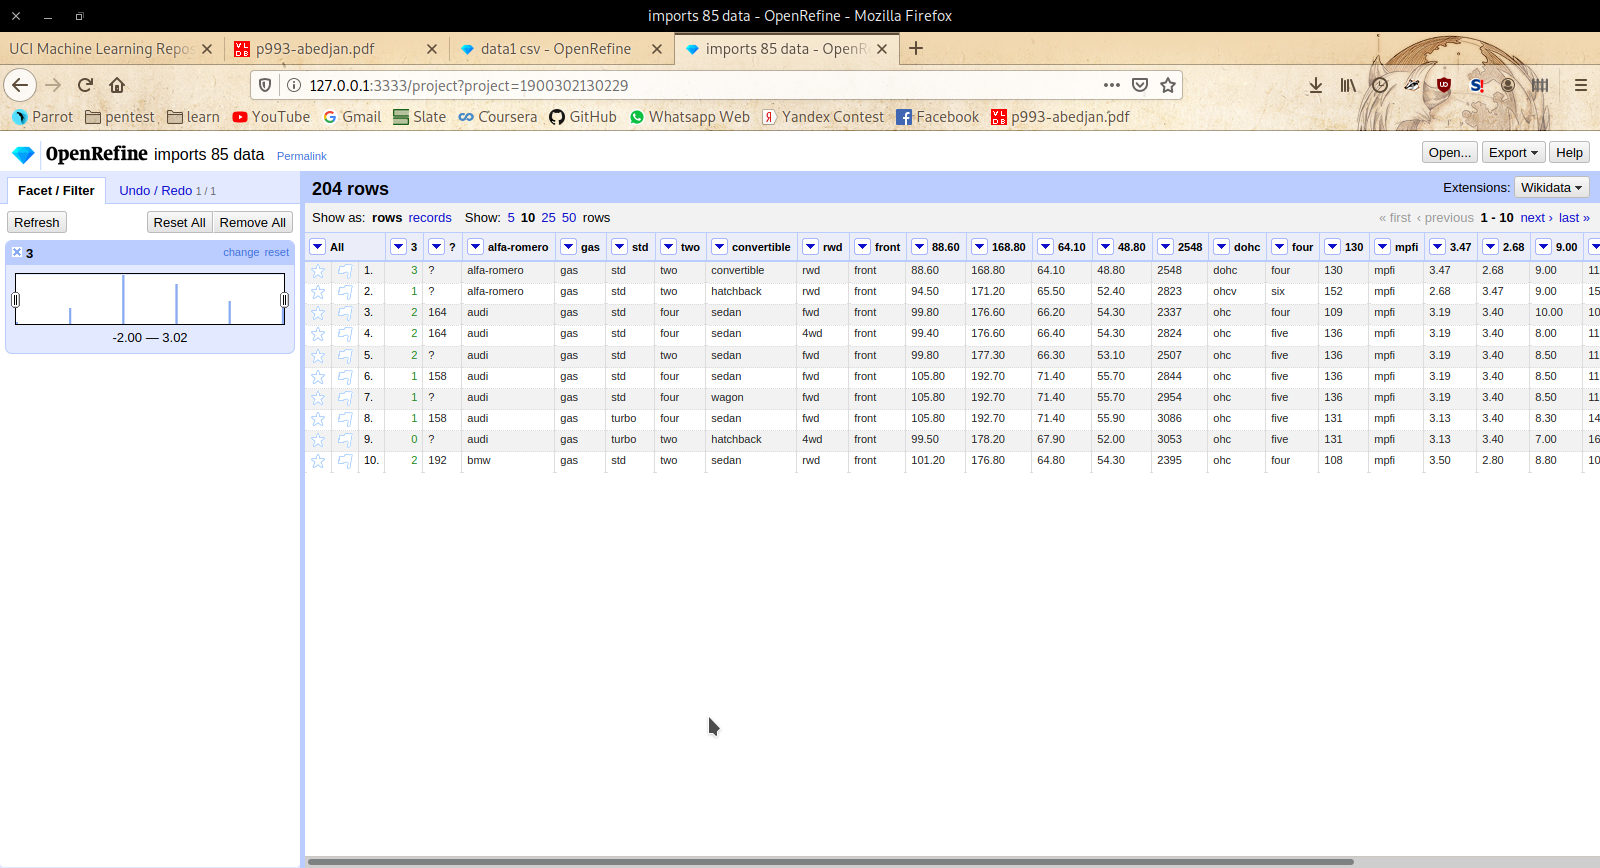
\includegraphics[width=\linewidth]{OpenRefine.png}
  \caption{OpenRefine Automobile dataset}
  \label{fig:OpenRefine}
\end{figure}

\subsubsection*{Knime}
Knime pronounced (ni-em) is graphical based data cleaning tool, somewhat like \emph{rapid miner} also able to implement models such as random forest. Running on Java runtime it works on a nodes based drag and drop structure opposed to the faucet based functionality in OpenRefine. Available through the GNU open source license \emph{Knime} is as easy to use as easily available. For the purpose of simplification and keeping within the specified limit we will applying the same configurations to both the dataset i.e. \textbf{automobile and locally generated dataset}. \\

\underline{Data cleaning in Knime}
\begin{enumerate}
	\item To add data to a project, we need to create a workflow first.
	\item Add a \emph{read csv} node to the workflow. Right click it to display further options out which we will select configure, or just hit shortcut F6.
	\item In the configure dialogue box direct the node to the data stored in the system, for now we will be working with a csv format, hence select csv file. Click \emph{Apply \textgreater Ok}. Remember to check \textbackslash uncheck row and column header as per the need.
	\item Right click on the node to display a dialogue box showing execute option and select it (shortcut F7). The node status will turn green and the uploaded data can now be displayed. String values present in a Interger column will automatically be removed and an empty cell be present to modify as per the user need.
	\item Next, drag in a node for statistics, not for our main purpose, but visualizing data is always preferred. 
	\item Connect the read csv node to the statistics nodes. Similarly this node can be executed and the table viewed.
	\item For data processing we will be filling in missing values next. Search for a missing values node and connect to the read csv node. The missing value node has a lot of configurations present for filling in missing values such as fill with mean of the column, previous value, next value or even mean average. You can even select different configuration for every column. Click Apply and then Ok after choosing your preferred settings.
	\item How about an integer to string conversion node? This node will unify all columns and make our dataset consistent. Simply configure by adding and removing columns to which the operation is to be implemented on and click execute.
\end{enumerate}

\begin{figure}
  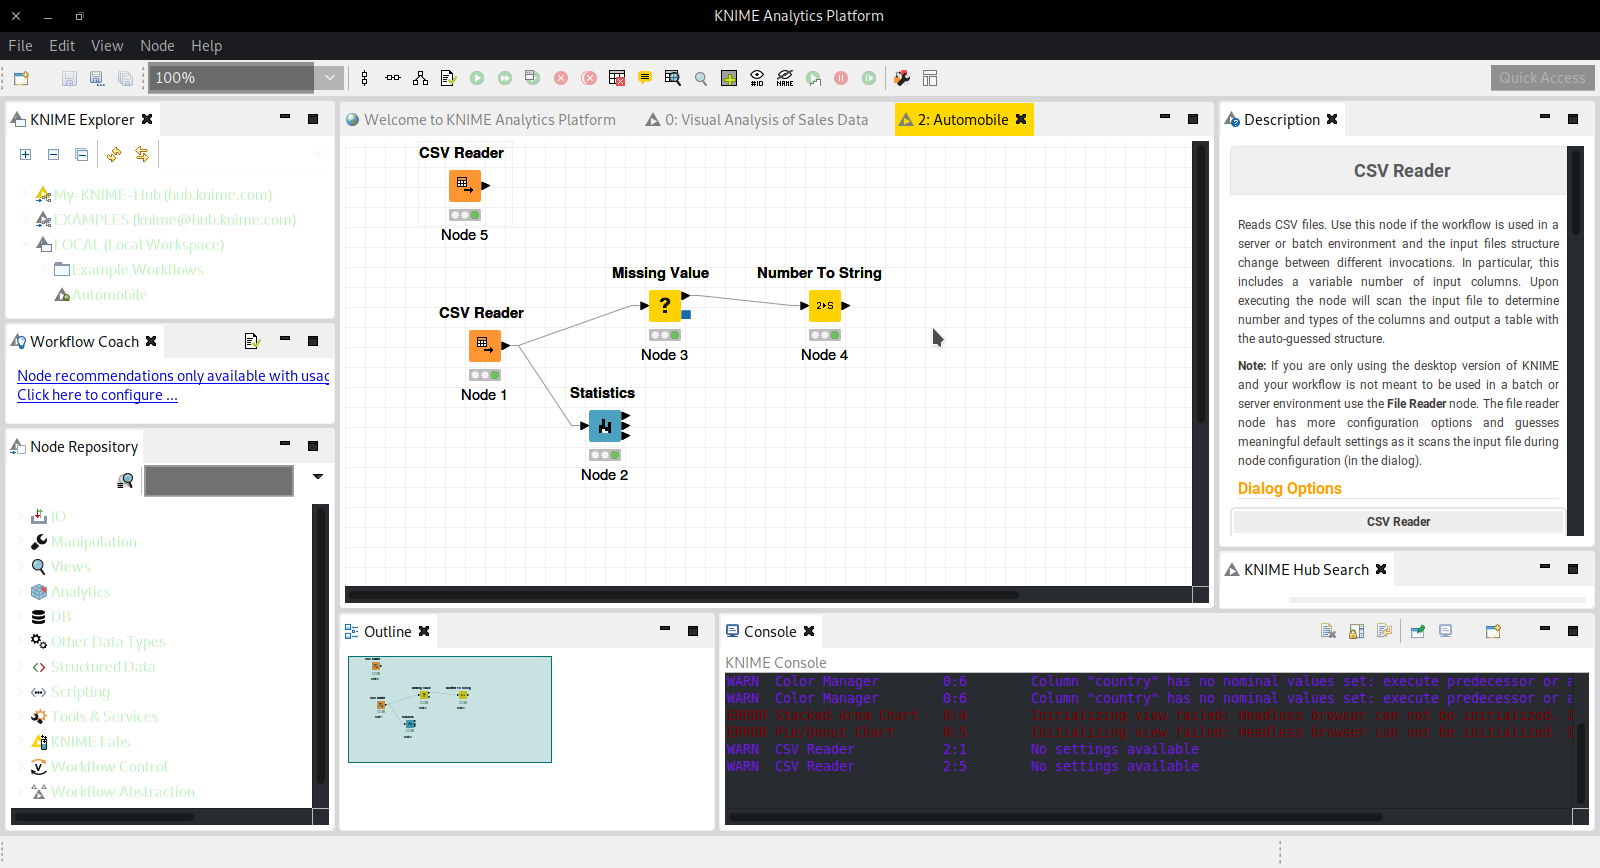
\includegraphics[width=\linewidth]{Knime.png}
  \caption{Knime workflow example}
  \label{fig:Knime Workflow}
\end{figure}

\end{document}
